\begin{enumerate}[label=\thesubsection.\arabic*.,ref=\thesubsection.\theenumi]
\numberwithin{equation}{enumi}

\item A dc amplifier having a single-pole response with pole frequency 10Hz and unity-gain frequency of 1MHz is operated in a loop whose frequency-independent feedback factor is 0.01. Find the low-frequency gain, the 3-dB frequency, and the unity-gain frequency of the closed-loop amplifier. By what factor does the pole shift?\\
\solution The open-loop gain of the amplifier is
\begin{align}
    G\brak{s}=\frac{A_{O}}{1+\frac{s}{\omega_p}}=\frac{A_{O}}{1+\frac{s}{2\pi.10}}
\end{align}
Given that unity gain frequency is 1MHz\\
Replacing $s$ with $\j\omega$ in this equation.
\begin{align}
    \abs{\frac{A_{O}}{1+\frac{\j.2\pi.10^6}{2\pi.10}}}&=1\\
    \abs{A_{O}}&=\abs{1+\j\frac{2\pi.10^6}{2\pi.10}}\\
    A_{O}&\approx10^5
\end{align}

\item Draw the bode plots of open-loop circuit\\
\solution
\begin{figure}[!h]
  \includegraphics[width=\columnwidth]{./figs/ee18btech11035_bode1.eps}
  \caption{Bode plots of Open-loop Transfer Function}
  \label{fig:ee18btech11035_bode1}
\end{figure}

Python code for above plot is
\begin{lstlisting}
codes/ee18btech11035_bode1.py
\end{lstlisting}

\item Design a Circuit for G\brak{s}\\
\solution Designing G\brak{s} Using Op-amp with DC gain of $10^5$ and a pole at 10Hz.

\begin{figure}[!ht]
    \begin{center}
		\resizebox{\columnwidth}{!}{\begin{circuitikz}[american]

\draw (2,2)  node[op amp] (OA) {};
\draw (OA.+) -- (0,1.5) to[vsourcesin, l= $V_{in}$] (0,0) node[ground](GND){};
\draw (OA.-) -- (0,2.5) node[ground, rotate=270](GND){};
\draw (3,2) -- (4,2) node[label={above:$V_{amp}$}]{};
\end{circuitikz}}
	\end{center}
\caption{}
\label{fig:ee18btech11035_G}
\end{figure}



\item Verify the gain using spice\\
\solution Netlist file for simulation:
\begin{lstlisting}
spice/ee18btech11035_spice1.net
\end{lstlisting}

\begin{figure}[!h]
  \includegraphics[width=\columnwidth]{./figs/ee18btech11035_spice1.eps}
  \caption{Spice Simulation of Open-loop Transfer Function}
  \label{fig:ee18btech11035_spice1}
\end{figure}


Python code for above plot:
\begin{lstlisting}
codes/ee18btech11035_spice1.py
\end{lstlisting}

\item Verification of step response of open-loop transfer function through python\\
\solution 
\begin{figure}[!h]
  \includegraphics[width=\columnwidth]{./figs/ee18btech11035_python1.eps}
  \caption{Python verification of Open-loop Transfer Function}
  \label{fig:ee18btech11035_pv1}
\end{figure}

Python code for above verification is 
\begin{lstlisting}
codes/ee18btech11035_pythonverify1.py
\end{lstlisting}


\item Add a feedback for above circuit with a feedback factor of 0.01 an calculate closed-loop transfer function\\
\solution $G\brak{s}=\frac{10^5}{1+\frac{s}{2\pi.10}}$ and $H\brak{s}=0.01$
\begin{align}
    T\brak{s}&=\frac{G\brak{s}}{1+G\brak{s}H\brak{s}}
\end{align}
\begin{align}
    T&=\frac{\frac{A_{O}}{1+A_{0}H\brak{s}}}{1+\frac{s}{20\pi\brak{1+A_{O}H\brak{s}}}}\\
    T\brak{s}&=\frac{99.90}{1+\frac{s}{2\pi.10010}}
\end{align}





Block diagram representation of the amplifier
\begin{figure}[!ht]
    \begin{center}
		\resizebox{\columnwidth}{!}{\tikzset{
        block/.style = {draw, rectangle,
            minimum height=1cm,
            minimum width=2cm},
        input/.style = {coordinate,node distance=1cm},
        output/.style = {coordinate,node distance=4cm},
        arrow/.style={draw, -latex,node distance=2cm},
        pinstyle/.style = {pin edge={latex-, black,node distance=2cm}},
        sum/.style = {draw, circle, node distance=1cm},
}

\begin{tikzpicture}[node distance=2.5cm,auto,>=latex']
  \node [input, name=input] {};
  \node [sum, right of=input] (sum) {};
  \node [block, right of = sum] (block1) {$G\brak{s}$};
  \node [block, below of= block1] (block2) {$H\brak{s}$};
  \node [output, right of= block1] (output) {};
  
  
  
  \draw [->] (input) -- node {$V_{in}$} (sum);
  \draw [->] (sum) -- node {} (block1);
  \draw [->] (block1) -- node [name =y] {$V_{out}$} (output);
  \draw [->] (y) |- node {} (block2);
  \draw [->] (block2) -| node [pos=0.99] {$-$} (sum);
\end{tikzpicture}
}
	\end{center}
\caption{}
\label{fig:ee18btech11035_block}
\end{figure}

\item Find the low frequency gain of the closed-loop amplifier.\\ 
\solution As frequency is low,substituting $s=0$\\
\begin{align}
    T\brak{0}&=\frac{G\brak{0}}{1+G\brak{0}H\brak{0}}\\
    &=\frac{10^5}{1+10^5.\brak{0.01}}\\
    &=99.900
\end{align}

\item Find the 3-dB frequency of the closed loop amplifier\\
\solution
\begin{align}
    T&=\frac{\frac{A_{O}}{1+A_{0}H\brak{s}}}{1+\frac{s}{20\pi\brak{1+A_{O}H\brak{s}}}}\\
    \text{3-dB frequency}&=20\pi.\brak{1+A_{O}H\brak{s}}\\
    &=20\pi.\brak{1+10^5.\brak{0.01}}\\
    &=62862.8rad/s=10.01kHz
\end{align}

\item Find the unity gain frequency of the closed loop amplifier\\
\solution Unity-gain frequency of the closed loop amplifier is obtained as follows
\begin{align}
    \abs{T}&=1\\
    \frac{A_{O}}{1+A_{O}H\brak{s}}&=\abs{1+\frac{\j\omega}{20\pi\brak{1+A_{O}H\brak{s}}}}\\
    99.900&=\abs{1+\frac{\j\omega}{62862.8}}\\
    \omega&=6279.649Krad/s=999.94kHz
\end{align}


\item By what factor does the pole shift?\\
\solution Open-loop pole is 10Hz and the Closed-loop pole is $20\pi.\brak{1+A_{O}H\brak{s}}$\\
\begin{align}
    \text{Pole-shift Factor}&=\frac{20\pi\brak{1+A_{O}H\brak{s}}}{20\pi}\\
    &=1+A_{O}H\brak{s}=1001
\end{align}



\item Design the feedback with $H\brak{s}=0.01$\\
\solution Designing Feedback circuit:\\
As,Feedback is a constant value designing it by using simple voltage divider circuit
\begin{figure}[!ht]
    \begin{center}
		\resizebox{\columnwidth}{!}{\begin{circuitikz}[american]
\ctikzset{tripoles/mos style/arrows}
\draw (1,2) to[short, -o] (0,2) node[label={above:$V_{out}$}]{};
\draw (1,2) to[R=$R_{f}$] (3,2) to[R=$R_{1}$] (3,0) node[ground](GND){};
\draw (3,2) to[short, -o] (4,2) node[label={above:$V_{f}$}]{};
\end{circuitikz}}
	\end{center}
\caption{}
\label{fig:ee18btech11035_feedback}
\end{figure}

\begin{align}
    \frac{V_{f}}{V_{out}}=\frac{R_{1}}{R_{1}+R_{f}}=H\brak{s}=0.01
\end{align}
Choosing $R_{1}$ as $10\ohm$ and $R_{f}$ as 990\ohm\\

Overall Circuit is as follows:
\begin{figure}[!ht]
    \begin{center}
		\resizebox{\columnwidth}{!}{\begin{circuitikz}[american]

\draw (2,2)  node[op amp] (OA) {};
\draw (OA.+) -- (0,1.5) to[vsourcesin, l= $V_{in}$] (0,0) node[ground](GND){};
\draw (OA.-) -- (0,2.5) node[label={below:$V_{f}$}]{} to[R,l_=$10\ohm$] (-2,2.5) node[ground](GND){};

\draw (3,2) -- (4.5,2) node[label={}]{} ;
\draw (4.5,2) -- (5.5,2) node[label={above:$V_{o}$}]{};
\draw (4.5,2) -- (4.5,4.5) to[R=$990\ohm$] (0,4.5) -- (0,2.5);
\end{circuitikz}}
	\end{center}
\caption{}
\label{fig:ee18btech11035_circuit}
\end{figure}


\begin{table}[!ht]
\centering
%%%%%%%%%%%%%%%%%%%%%%%%%%%%%%%%%%%%%%%%%%%%%%%%%%%%%%%%%%%%%%%%%%%%%%
%%                                                                  %%
%%  This is the header of a LaTeX2e file exported from Gnumeric.    %%
%%                                                                  %%
%%  This file can be compiled as it stands or included in another   %%
%%  LaTeX document. The table is based on the longtable package so  %%
%%  the longtable options (headers, footers...) can be set in the   %%
%%  preamble section below (see PRAMBLE).                           %%
%%                                                                  %%
%%  To include the file in another, the following two lines must be %%
%%  in the including file:                                          %%
%%        \def\inputGnumericTable{}                                 %%
%%  at the beginning of the file and:                               %%
%%        \input{name-of-this-file.tex}                             %%
%%  where the table is to be placed. Note also that the including   %%
%%  file must use the following packages for the table to be        %%
%%  rendered correctly:                                             %%
%%    \usepackage[latin1]{inputenc}                                 %%
%%    \usepackage{color}                                            %%
%%    \usepackage{array}                                            %%
%%    \usepackage{longtable}                                        %%
%%    \usepackage{calc}                                             %%
%%    \usepackage{multirow}                                         %%
%%    \usepackage{hhline}                                           %%
%%    \usepackage{ifthen}                                           %%
%%  optionally (for landscape tables embedded in another document): %%
%%    \usepackage{lscape}                                           %%
%%                                                                  %%
%%%%%%%%%%%%%%%%%%%%%%%%%%%%%%%%%%%%%%%%%%%%%%%%%%%%%%%%%%%%%%%%%%%%%%



%%  This section checks if we are begin input into another file or  %%
%%  the file will be compiled alone. First use a macro taken from   %%
%%  the TeXbook ex 7.7 (suggestion of Han-Wen Nienhuys).            %%
\def\ifundefined#1{\expandafter\ifx\csname#1\endcsname\relax}


%%  Check for the \def token for inputed files. If it is not        %%
%%  defined, the file will be processed as a standalone and the     %%
%%  preamble will be used.                                          %%
\ifundefined{inputGnumericTable}

%%  We must be able to close or not the document at the end.        %%
	\def\gnumericTableEnd{\end{document}}


%%%%%%%%%%%%%%%%%%%%%%%%%%%%%%%%%%%%%%%%%%%%%%%%%%%%%%%%%%%%%%%%%%%%%%
%%                                                                  %%
%%  This is the PREAMBLE. Change these values to get the right      %%
%%  paper size and other niceties.                                  %%
%%                                                                  %%
%%%%%%%%%%%%%%%%%%%%%%%%%%%%%%%%%%%%%%%%%%%%%%%%%%%%%%%%%%%%%%%%%%%%%%

	\documentclass[12pt%
			  %,landscape%
                    ]{report}
       \usepackage[latin1]{inputenc}
       \usepackage{fullpage}
       \usepackage{color}
       \usepackage{array}
       \usepackage{longtable}
       \usepackage{calc}
       \usepackage{multirow}
       \usepackage{hhline}
       \usepackage{ifthen}


%%  End of the preamble for the standalone. The next section is for %%
%%  documents which are included into other LaTeX2e files.          %%
\else

%%  We are not a stand alone document. For a regular table, we will %%
%%  have no preamble and only define the closing to mean nothing.   %%
    \def\gnumericTableEnd{}

%%  If we want landscape mode in an embedded document, comment out  %%
%%  the line above and uncomment the two below. The table will      %%
%%  begin on a new page and run in landscape mode.                  %%
%       \def\gnumericTableEnd{\end{landscape}}
%       \begin{landscape}


%%  End of the else clause for this file being \input.              %%
\fi

%%%%%%%%%%%%%%%%%%%%%%%%%%%%%%%%%%%%%%%%%%%%%%%%%%%%%%%%%%%%%%%%%%%%%%
%%                                                                  %%
%%  The rest is the gnumeric table, except for the closing          %%
%%  statement. Changes below will alter the table's appearance.     %%
%%                                                                  %%
%%%%%%%%%%%%%%%%%%%%%%%%%%%%%%%%%%%%%%%%%%%%%%%%%%%%%%%%%%%%%%%%%%%%%%

\providecommand{\gnumericmathit}[1]{#1} 
%%  Uncomment the next line if you would like your numbers to be in %%
%%  italics if they are italizised in the gnumeric table.           %%
%\renewcommand{\gnumericmathit}[1]{\mathit{#1}}
\providecommand{\gnumericPB}[1]%
{\let\gnumericTemp=\\#1\let\\=\gnumericTemp\hspace{0pt}}
 \ifundefined{gnumericTableWidthDefined}
        \newlength{\gnumericTableWidth}
        \newlength{\gnumericTableWidthComplete}
        \newlength{\gnumericMultiRowLength}
        \global\def\gnumericTableWidthDefined{}
 \fi
%% The following setting protects this code from babel shorthands.  %%
 \ifthenelse{\isundefined{\languageshorthands}}{}{\languageshorthands{english}}
%%  The default table format retains the relative column widths of  %%
%%  gnumeric. They can easily be changed to c, r or l. In that case %%
%%  you may want to comment out the next line and uncomment the one %%
%%  thereafter                                                      %%
\providecommand\gnumbox{\makebox[0pt]}
%%\providecommand\gnumbox[1][]{\makebox}

%% to adjust positions in multirow situations                       %%
\setlength{\bigstrutjot}{\jot}
\setlength{\extrarowheight}{\doublerulesep}

%%  The \setlongtables command keeps column widths the same across  %%
%%  pages. Simply comment out next line for varying column widths.  %%
\setlongtables

\setlength\gnumericTableWidth{%
	75pt+%
	75pt+%
0pt}
\def\gumericNumCols{2}
\setlength\gnumericTableWidthComplete{\gnumericTableWidth+%
         \tabcolsep*\gumericNumCols*2+\arrayrulewidth*\gumericNumCols}
\ifthenelse{\lengthtest{\gnumericTableWidthComplete > \linewidth}}%
         {\def\gnumericScale{\ratio{\linewidth-%
                        \tabcolsep*\gumericNumCols*2-%
                        \arrayrulewidth*\gumericNumCols}%
{\gnumericTableWidth}}}%
{\def\gnumericScale{1}}

%%%%%%%%%%%%%%%%%%%%%%%%%%%%%%%%%%%%%%%%%%%%%%%%%%%%%%%%%%%%%%%%%%%%%%
%%                                                                  %%
%% The following are the widths of the various columns. We are      %%
%% defining them here because then they are easier to change.       %%
%% Depending on the cell formats we may use them more than once.    %%
%%                                                                  %%
%%%%%%%%%%%%%%%%%%%%%%%%%%%%%%%%%%%%%%%%%%%%%%%%%%%%%%%%%%%%%%%%%%%%%%

\ifthenelse{\isundefined{\gnumericColA}}{\newlength{\gnumericColA}}{}\settowidth{\gnumericColA}{\begin{tabular}{@{}p{75pt*\gnumericScale}@{}}x\end{tabular}}
\ifthenelse{\isundefined{\gnumericColB}}{\newlength{\gnumericColB}}{}\settowidth{\gnumericColB}{\begin{tabular}{@{}p{75pt*\gnumericScale}@{}}x\end{tabular}}

\begin{tabular}[c]{%
	b{\gnumericColA}%
	b{\gnumericColB}%
	}

%%%%%%%%%%%%%%%%%%%%%%%%%%%%%%%%%%%%%%%%%%%%%%%%%%%%%%%%%%%%%%%%%%%%%%
%%  The longtable options. (Caption, headers... see Goosens, p.124) %%
%	\caption{The Table Caption.}             \\	%
% \hline	% Across the top of the table.
%%  The rest of these options are table rows which are placed on    %%
%%  the first, last or every page. Use \multicolumn if you want.    %%

%%  Header for the first page.                                      %%
%	\multicolumn{3}{c}{The First Header} \\ \hline 
%	\multicolumn{1}{c}{colTag}	%Column 1
%	&\multicolumn{1}{c}{colTag}	%Column 2
%	&\multicolumn{1}{c}{colTag}	\\ \hline %Last column
%	\endfirsthead

%%  The running header definition.                                  %%
%	\hline
%	\multicolumn{3}{l}{\ldots\small\slshape continued} \\ \hline
%	\multicolumn{1}{c}{colTag}	%Column 1
%	&\multicolumn{1}{c}{colTag}	%Column 2
%	&\multicolumn{1}{c}{colTag}	\\ \hline %Last column
%	\endhead

%%  The running footer definition.                                  %%
%	\hline
%	\multicolumn{3}{r}{\small\slshape continued\ldots} \\
%	\endfoot

%%  The ending footer definition.                                   %%
%	\multicolumn{3}{c}{That's all folks} \\ \hline 
%	\endlastfoot
%%%%%%%%%%%%%%%%%%%%%%%%%%%%%%%%%%%%%%%%%%%%%%%%%%%%%%%%%%%%%%%%%%%%%%

\hhline{|-|-}
	 \multicolumn{1}{|p{\gnumericColA}|}%
	{\gnumericPB{\centering}Circuit Element}
	&\multicolumn{1}{p{\gnumericColB}|}%
	{\gnumericPB{\centering}Parameter Value}
	
\\
\hhline{|--|}
	 \multicolumn{1}{|p{\gnumericColA}|}%
	{\gnumericPB{\centering}Op-amp Gain}
	&\multicolumn{1}{p{\gnumericColB}|}%
	{\gnumericPB{\centering}$10^5$}

\\
\hhline{|--|}
	 \multicolumn{1}{|p{\gnumericColA}|}%
	{\gnumericPB{\centering}Op-amp pole}
	&\multicolumn{1}{p{\gnumericColB}|}%
	{\gnumericPB{\centering}$10Hz$}


\\
\hhline{|--|}
	 \multicolumn{1}{|p{\gnumericColA}|}%
	{\gnumericPB{\centering}$R_{1}$}
	&\multicolumn{1}{p{\gnumericColB}|}%
	{\gnumericPB{\centering}$10\ohm$}
\\
\hhline{|--|}
	 \multicolumn{1}{|p{\gnumericColA}|}%
	{\gnumericPB{\centering}$R_{f}$}
	&\multicolumn{1}{p{\gnumericColB}|}%
	{\gnumericPB{\centering}$990\ohm$}




\\

\hhline{|-|-}
\end{tabular}

\ifthenelse{\isundefined{\languageshorthands}}{}{\languageshorthands{\languagename}}
\gnumericTableEnd
\caption{}
\label{table:ee18btech11035_table1}
\end{table}


\item Draw the Bode plots of closed-loop circuit\\
\solution
\begin{figure}[!h]
  \includegraphics[width=\columnwidth]{./figs/ee18btech11035_bode2.eps}
  \caption{Bode plots of Closed-loop Transfer Function}
  \label{fig:ee18btech11035_bode2}
\end{figure}

Python code for above plot is
\begin{lstlisting}
codes/ee18btech11035_bode2.py
\end{lstlisting}



\item Verify the gain of closed loop Circuit using spice\\
\solution Follow the Instructions for SPICE simulation:
\begin{lstlisting}
spice/README.md
\end{lstlisting}
Netlist file for simulation:
\begin{lstlisting}
spice/ee18btech11035_spice2.net
\end{lstlisting}

\begin{figure}[!h]
  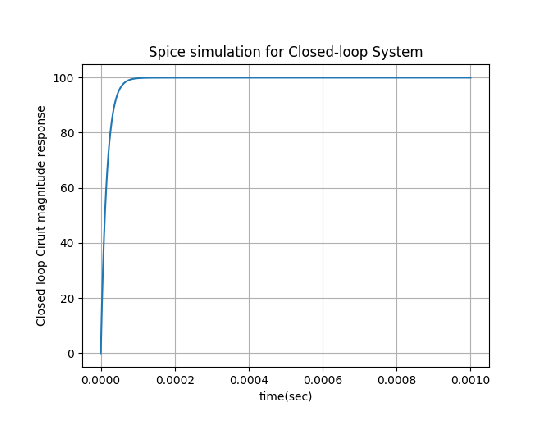
\includegraphics[width=\columnwidth]{./figs/ee18btech11035_spice2.eps}
  \caption{Spice simulation of Closed-loop Transfer Function}
  \label{fig:ee18btech11035_spice2}
\end{figure}


Pyhton code for above plot:
\begin{lstlisting}
codes/ee18btech11035_spice2.py
\end{lstlisting}

\item Verification of step response of open-loop transfer function through python\\
\solution 

\begin{figure}[!h]
  \includegraphics[width=\columnwidth]{./figs/ee18btech11035_python2.eps}
  \caption{Python verification of closed-loop Transfer Function}
  \label{fig:ee18btech11035_pv2}
\end{figure}


Python code for above verification is 
\begin{lstlisting}
codes/ee18btech11035_pythonverify2.py
\end{lstlisting}




\item Tabulating DC Gain,Bandwidth and Gain bandwidth product\\
\solution
Observing the fig:\eqref{fig:ee18btech11035_bode1} and fig:\eqref{fig:ee18btech11035_bode2} to get DC Gain and Bandwidth
\begin{table}[!ht]
\centering


%%  This section checks if we are begin input into another file or  %%
%%  the file will be compiled alone. First use a macro taken from   %%
%%  the TeXbook ex 7.7 (suggestion of Han-Wen Nienhuys).            %%
\def\ifundefined#1{\expandafter\ifx\csname#1\endcsname\relax}


%%  Check for the \def token for inputed files. If it is not        %%
%%  defined, the file will be processed as a standalone and the     %%
%%  preamble will be used.                                          %%
\ifundefined{inputGnumericTable}

%%  We must be able to close or not the document at the end.        %%
	\def\gnumericTableEnd{\end{document}}


%%%%%%%%%%%%%%%%%%%%%%%%%%%%%%%%%%%%%%%%%%%%%%%%%%%%%%%%%%%%%%%%%%%%%%
%%                                                                  %%
%%  This is the PREAMBLE. Change these values to get the right      %%
%%  paper size and other niceties.                                  %%
%%                                                                  %%
%%%%%%%%%%%%%%%%%%%%%%%%%%%%%%%%%%%%%%%%%%%%%%%%%%%%%%%%%%%%%%%%%%%%%%

	\documentclass[12pt%
			  %,landscape%
                    ]{report}
       \usepackage[latin1]{inputenc}
       \usepackage{fullpage}
       \usepackage{color}
       \usepackage{array}
       \usepackage{longtable}
       \usepackage{calc}
       \usepackage{multirow}
       \usepackage{hhline}
       \usepackage{ifthen}
%%  End of the preamble for the standalone. The next section is for %%
%%  documents which are included into other LaTeX2e files.          %%
\else

%%  We are not a stand alone document. For a regular table, we will %%
%%  have no preamble and only define the closing to mean nothing.   %%
    \def\gnumericTableEnd{}

%%  If we want landscape mode in an embedded document, comment out  %%
%%  the line above and uncomment the two below. The table will      %%
%%  begin on a new page and run in landscape mode.                  %%
%       \def\gnumericTableEnd{\end{landscape}}
%       \begin{landscape}


%%  End of the else clause for this file being \input.              %%
\fi

%%%%%%%%%%%%%%%%%%%%%%%%%%%%%%%%%%%%%%%%%%%%%%%%%%%%%%%%%%%%%%%%%%%%%%
%%                                                                  %%
%%  The rest is the gnumeric table, except for the closing          %%
%%  statement. Changes below will alter the table's appearance.     %%
%%                                                                  %%
%%%%%%%%%%%%%%%%%%%%%%%%%%%%%%%%%%%%%%%%%%%%%%%%%%%%%%%%%%%%%%%%%%%%%%

\providecommand{\gnumericmathit}[1]{#1} 
%%  Uncomment the next line if you would like your numbers to be in %%
%%  italics if they are italizised in the gnumeric table.           %%
%\renewcommand{\gnumericmathit}[1]{\mathit{#1}}
\providecommand{\gnumericPB}[1]%
{\let\gnumericTemp=\\#1\let\\=\gnumericTemp\hspace{0pt}}
 \ifundefined{gnumericTableWidthDefined}
        \newlength{\gnumericTableWidth}
        \newlength{\gnumericTableWidthComplete}
        \newlength{\gnumericMultiRowLength}
        \global\def\gnumericTableWidthDefined{}
 \fi
%% The following setting protects this code from babel shorthands.  %%
 \ifthenelse{\isundefined{\languageshorthands}}{}{\languageshorthands{english}}
%%  The default table format retains the relative column widths of  %%
%%  gnumeric. They can easily be changed to c, r or l. In that case %%
%%  you may want to comment out the next line and uncomment the one %%
%%  thereafter                                                      %%
\providecommand\gnumbox{\makebox[0pt]}
%%\providecommand\gnumbox[1][]{\makebox}

%% to adjust positions in multirow situations                       %%
\setlength{\bigstrutjot}{\jot}
\setlength{\extrarowheight}{\doublerulesep}

%%  The \setlongtables command keeps column widths the same across  %%
%%  pages. Simply comment out next line for varying column widths.  %%
\setlongtables

\setlength\gnumericTableWidth{%
	50pt+%
	50pt+%
	50pt+%
0pt}
\def\gumericNumCols{3}
\setlength\gnumericTableWidthComplete{\gnumericTableWidth+%
         \tabcolsep*\gumericNumCols*2+\arrayrulewidth*\gumericNumCols}
\ifthenelse{\lengthtest{\gnumericTableWidthComplete > \linewidth}}%
         {\def\gnumericScale{\ratio{\linewidth-%
                        \tabcolsep*\gumericNumCols*2-%
                        \arrayrulewidth*\gumericNumCols}%
{\gnumericTableWidth}}}%
{\def\gnumericScale{1}}

%%%%%%%%%%%%%%%%%%%%%%%%%%%%%%%%%%%%%%%%%%%%%%%%%%%%%%%%%%%%%%%%%%%%%%
%%                                                                  %%
%% The following are the widths of the various columns. We are      %%
%% defining them here because then they are easier to change.       %%
%% Depending on the cell formats we may use them more than once.    %%
%%                                                                  %%
%%%%%%%%%%%%%%%%%%%%%%%%%%%%%%%%%%%%%%%%%%%%%%%%%%%%%%%%%%%%%%%%%%%%%%

\ifthenelse{\isundefined{\gnumericColA}}{\newlength{\gnumericColA}}{}\settowidth{\gnumericColA}{\begin{tabular}{@{}p{50pt*\gnumericScale}@{}}x\end{tabular}}
\ifthenelse{\isundefined{\gnumericColB}}{\newlength{\gnumericColB}}{}\settowidth{\gnumericColB}{\begin{tabular}{@{}p{60pt*\gnumericScale}@{}}x\end{tabular}}
\ifthenelse{\isundefined{\gnumericColC}}{\newlength{\gnumericColC}}{}\settowidth{\gnumericColC}{\begin{tabular}{@{}p{60pt*\gnumericScale}@{}}x\end{tabular}}

\begin{tabular}[c]{%
	b{\gnumericColA}%
	b{\gnumericColB}%
	b{\gnumericColC}%
	}

%%%%%%%%%%%%%%%%%%%%%%%%%%%%%%%%%%%%%%%%%%%%%%%%%%%%%%%%%%%%%%%%%%%%%%
%%  The longtable options. (Caption, headers... see Goosens, p.124) %%
%	\caption{The Table Caption.}             \\	%
% \hline	% Across the top of the table.
%%  The rest of these options are table rows which are placed on    %%
%%  the first, last or every page. Use \multicolumn if you want.    %%

%%  Header for the first page.                                      %%
%	\multicolumn{3}{c}{The First Header} \\ \hline 
%	\multicolumn{1}{c}{colTag}	%Column 1
%	&\multicolumn{1}{c}{colTag}	%Column 2
%	&\multicolumn{1}{c}{colTag}	\\ \hline %Last column
%	\endfirsthead

%%  The running header definition.                                  %%
%	\hline
%	\multicolumn{3}{l}{\ldots\small\slshape continued} \\ \hline
%	\multicolumn{1}{c}{colTag}	%Column 1
%	&\multicolumn{1}{c}{colTag}	%Column 2
%	&\multicolumn{1}{c}{colTag}	\\ \hline %Last column
%	\endhead

%%  The running footer definition.                                  %%
%	\hline
%	\multicolumn{3}{r}{\small\slshape continued\ldots} \\
%	\endfoot

%%  The ending footer definition.                                   %%
%	\multicolumn{3}{c}{That's all folks} \\ \hline 
%	\endlastfoot
%%%%%%%%%%%%%%%%%%%%%%%%%%%%%%%%%%%%%%%%%%%%%%%%%%%%%%%%%%%%%%%%%%%%%%

\hhline{|-|-|-}
	 \multicolumn{1}{|p{\gnumericColA}|}%
	{\gnumericPB{\centering}\textbf{}}
	&\multicolumn{1}{p{\gnumericColB}|}%
	{\gnumericPB{\centering}\textbf{$G\brak{s}$}}
	&\multicolumn{1}{p{\gnumericColC}|}%
	{\gnumericPB{\centering}\textbf{$T\brak{s}$}}

	
\\


\hhline{|---|}
	 \multicolumn{1}{|p{\gnumericColA}|}%
	{\gnumericPB{\centering}{Gain}}
	&\multicolumn{1}{p{\gnumericColB}|}%
	{\gnumericPB{\centering}{$10^5$}}
	&\multicolumn{1}{p{\gnumericColC}|}%
	{\gnumericPB{\centering}{$99.9$}}

\\
\hhline{|---|}
	 \multicolumn{1}{|p{\gnumericColA}|}%
	{\gnumericPB{\centering}{Bandwidth}}
	&\multicolumn{1}{p{\gnumericColB}|}%
	{\gnumericPB{\centering}{$20\pi$}}
	&\multicolumn{1}{p{\gnumericColC}|}%
	{\gnumericPB{\centering}{$20\pi.1001$}}

\\
\hhline{|---|}
	 \multicolumn{1}{|p{\gnumericColA}|}%
	{\gnumericPB{\centering}Gain bandwidth product}
	&\multicolumn{1}{p{\gnumericColB}|}%
	{\gnumericPB{\centering}{$2\pi.10^6$}}
	&\multicolumn{1}{p{\gnumericColC}|}%
	{\gnumericPB{\centering}{$2\pi.10^6$}}




\\
\hhline{|-|-|-|}
\end{tabular}

\ifthenelse{\isundefined{\languageshorthands}}{}{\languageshorthands{\languagename}}
\gnumericTableEnd
\caption{}
\label{table:ee18btech11035_table2}
\end{table}

Therefore,By using feedback we can get desired Gain of an amplifier while maintaining constant Gain Bandwidth product(Only for a first-order op-amp).


\end{enumerate}
